\chapter{Descripción de la propuesta}
\label{cap:propuesta}

Este capítulo describe en detalle el sistema propuesto: su arquitectura general, las fuentes de datos utilizadas, el proceso de extracción y transformación de datos, el modelado de la red viaria, el diseño de la función de coste de seguridad y la implementación del enrutamiento. El sistema se denomina en adelante \textbf{SafeMaps-Madrid}.

% -----------------------------------------------------------------------
% 3.1 VISIÓN GENERAL DEL SISTEMA
% -----------------------------------------------------------------------
\section{Visión general del sistema}
\label{sec:vision_general}

SafeMaps-Madrid es un sistema de cálculo de rutas seguras para peatones en el entorno urbano de Madrid. Su objetivo es ofrecer al usuario, dado un origen y un destino, una ruta que minimice la exposición a factores de riesgo urbano, como alternativa informada a la ruta más corta convencional.

El sistema se articula en torno a cuatro componentes principales, cuya interacción se ilustra en la Figura~\ref{fig:arquitectura}:

\begin{enumerate}
    \item \textbf{Pipeline ETL}: proceso de extracción, transformación y carga de los datos de las fuentes de riesgo (iluminación pública, accidentalidad peatonal y vulnerabilidad territorial), así como de la red viaria y los distritos administrativos, en la base de datos espacial.
    \item \textbf{Base de datos espacial}: instancia PostgreSQL/PostGIS que almacena la red viaria de Madrid, los indicadores de riesgo georreferenciados y las aristas del grafo con sus pesos de seguridad calculados.
    \item \textbf{Motor de enrutamiento}: extensión pgRouting sobre la base de datos espacial, que implementa el algoritmo de Dijkstra sobre el grafo ponderado para calcular la ruta de menor coste de seguridad.
    \item \textbf{Visor cartográfico web}: interfaz de usuario desarrollada con Leaflet y un backend en Flask que permite introducir origen y destino —escribiendo una dirección, mediante geolocalización o haciendo clic en el mapa—, lanzar la consulta de enrutamiento y visualizar la ruta segura junto a la ruta más corta sobre un mapa de Madrid.
\end{enumerate}

\begin{figure}[h]
\centering
\begin{tikzpicture}[
    font=\small,
    comp/.style={rectangle, rounded corners, draw=black, thick, fill=gray!10,
        minimum width=7.6cm, minimum height=1.15cm, align=center},
    ctx/.style={rectangle, rounded corners, draw=black, dashed, fill=white,
        minimum width=7.6cm, minimum height=0.9cm, align=center},
    arr/.style={-{Latex[length=2.2mm]}, thick},
    lbl/.style={font=\scriptsize, align=center, fill=white, inner sep=1pt}
]

\node[ctx] (fuentes) {Fuentes de datos abiertas\\
    \scriptsize OpenStreetMap · Geoportal de Madrid · Datos Abiertos Madrid};

\node[comp, below=1.3cm of fuentes] (etl) {Pipeline ETL\\
    \scriptsize \texttt{scripts/01\_}--\texttt{06\_} (Python, osmnx, GeoPandas)};

\node[comp, below=1.3cm of etl] (bd) {Base de datos espacial\\
    \scriptsize PostgreSQL 16 + PostGIS --- \texttt{safe\_maps}};

\node[comp, below=1.3cm of bd] (routing) {Motor de enrutamiento\\
    \scriptsize pgRouting --- \texttt{pgr\_dijkstra}};

\node[comp, below=1.3cm of routing] (visor) {Visor cartográfico web\\
    \scriptsize Flask (backend) + Leaflet (frontend)};

\node[ctx, below=1.3cm of visor] (usuario) {Usuario};

\draw[arr] (fuentes) -- (etl) node[lbl, midway] {extracción};
\draw[arr] (etl) -- (bd) node[lbl, midway] {carga\\ \scriptsize SQLAlchemy};
\draw[arr] (bd) -- (routing) node[lbl, midway] {consulta ponderada\\ \scriptsize \texttt{cost} / \texttt{cost\_seguro}};
\draw[arr] (routing) -- (visor) node[lbl, midway] {\texttt{calcular\_ruta()}};
\draw[arr] (visor) -- (usuario) node[lbl, midway] {HTTP / JSON};

\end{tikzpicture}
\caption{Arquitectura general del sistema SafeMaps-Madrid. Los recuadros sólidos son los cuatro componentes principales descritos en esta sección; los recuadros discontinuos representan el contexto externo (fuentes de datos y usuario final). El motor de enrutamiento se ejecuta como extensión dentro de la misma instancia de PostgreSQL que la base de datos espacial.}
\label{fig:arquitectura}
\end{figure}

A diferencia del planteamiento inicial del proyecto, la versión implementada de SafeMaps-Madrid \textbf{no distingue franjas horarias}: el coste de seguridad de cada arista es único e independiente de la hora del día. Esta simplificación se adoptó por dos motivos. Primero, los datos de accidentalidad disponibles no permiten una segmentación diurna/nocturna suficientemente robusta como para calcular dos indicadores fiables sin perder densidad muestral en buena parte de la red. Segundo, al no disponerse de un indicador de criminalidad real (véase la Sección~\ref{subsec:vulnerabilidad_datos}), el argumento principal para justificar la ponderación temporal —la variación día/noche del riesgo de criminalidad documentada por Levy et al. \cite{levy2020}— pierde parte de su fundamento en este sistema. La incorporación de una dimensión temporal se plantea como línea de trabajo futuro en el Capítulo~\ref{cap:conclusiones}.

% -----------------------------------------------------------------------
% 3.2 FUENTES DE DATOS
% -----------------------------------------------------------------------
\section{Fuentes de datos}
\label{sec:fuentes_datos}

El sistema integra cinco fuentes de datos georreferenciados, todas ellas de acceso público y libre:

\subsection{Red viaria: OpenStreetMap}
\label{subsec:osm_datos}

La red viaria de Madrid se obtiene de \textbf{OpenStreetMap} (OSM), el proyecto colaborativo de cartografía libre, a través de la biblioteca Python \texttt{osmnx} \cite{boeing2017}, que consulta la API de Overpass y descarga directamente el subgrafo peatonal (\texttt{network\_type="walk"}) correspondiente al municipio de Madrid. Esta aproximación evita la descarga y el procesado manual de un extracto \texttt{.osm.pbf} completo de la región, ya que \texttt{osmnx} filtra en origen los tipos de vía no transitables a pie y devuelve directamente un grafo topológicamente conexo, con sus atributos de tipo de vía, nombre y geometría.

\subsection{Iluminación pública: Geoportal del Ayuntamiento de Madrid}
\label{subsec:iluminacion_datos}

Los datos de iluminación pública se obtienen del \textbf{Geoportal del Ayuntamiento de Madrid} \cite{madridgeoportal}, que publica la ubicación de las unidades luminosas de la red de alumbrado público en formato Shapefile. Cada punto de luz incluye su posición geográfica, lo que permite calcular la densidad de iluminación en el entorno de cada segmento de calle.

\subsection{Vulnerabilidad territorial: Índice Iguala Madrid}
\label{subsec:vulnerabilidad_datos}

El planteamiento inicial del proyecto contemplaba el uso de un indicador de \textbf{criminalidad} por distrito. Sin embargo, el Ayuntamiento de Madrid no publica estadísticas de delitos georreferenciadas ni desagregadas por zona: los datos de criminalidad los custodia el Ministerio del Interior a través del Sistema Estadístico de Criminalidad, y por razones de protección de datos y de la propia investigación policial no se difunden con el nivel de detalle geográfico que requeriría este sistema. Ante esta limitación, se ha optado por sustituir el indicador de criminalidad por un indicador de \textbf{vulnerabilidad territorial}, obtenido del \textbf{Índice Iguala Madrid} \cite{madridiguala}, un estudio del Ayuntamiento que calcula, para cada uno de los 21 distritos de la ciudad, un índice compuesto de vulnerabilidad a partir de variables socioeconómicas (renta media, tasa de población extranjera, envejecimiento, entre otras) agregadas en cinco esferas —bienestar social e igualdad, medio ambiente urbano y movilidad, educación y cultura, economía y empleo, y salud—. Se utiliza el \textit{Índice de Vulnerabilidad Territorial Agregado} del año más reciente disponible (2024) como indicador de referencia.

Se trata de una variable \textit{proxy} y no de una medida directa de criminalidad: un distrito con mayor vulnerabilidad territorial no implica necesariamente una mayor tasa de delitos, aunque la literatura sobre desigualdad urbana asocia habitualmente la vulnerabilidad socioeconómica con una peor percepción de seguridad y con determinados factores de riesgo ambiental (peor mantenimiento del espacio público, menor vigilancia informal). Esta limitación se discute con más detalle en el Capítulo~\ref{cap:conclusiones}.

\subsection{Distritos administrativos: Geoportal del Ayuntamiento de Madrid}
\label{subsec:distritos_datos}

Dado que tanto los datos de accidentalidad como el Índice Iguala están agregados a nivel de distrito, es necesario disponer de los límites administrativos de los 21 distritos de Madrid para poder asignar cada segmento de la red viaria al distrito al que pertenece. Estos límites se obtienen también del \textbf{Geoportal del Ayuntamiento de Madrid} \cite{madridgeoportal}, en formato Shapefile.

\subsection{Accidentes con víctimas peatonales: Portal de Datos Abiertos de Madrid}
\label{subsec:accidentes_datos}

Los datos de accidentalidad se obtienen del \textbf{Portal de Datos Abiertos del Ayuntamiento de Madrid} \cite{madridopendata}, que publica el registro anual de accidentes de tráfico con víctimas en la ciudad de Madrid a nivel de persona implicada (un accidente con varios implicados genera varios registros). Cada registro incluye la ubicación del accidente (coordenadas UTM), la fecha y hora, el tipo de accidente, el tipo de persona implicada (conductor, pasajero o peatón) y la gravedad de las lesiones. Se utilizan los datos correspondientes a los años 2023, 2024 y 2025.

% -----------------------------------------------------------------------
% 3.3 PROCESO ETL
% -----------------------------------------------------------------------
\section{Proceso ETL}
\label{sec:etl}

El proceso ETL (Extract, Transform, Load) es la fase de preparación de datos previa a su integración en la base de datos espacial. Se implementa como una secuencia de scripts de Python numerados según su orden de ejecución (\texttt{scripts/01\_*.py} a \texttt{scripts/06\_*.py}), cada uno responsable de una fuente de datos y \textbf{idempotente}: comprueba si los datos ya están cargados antes de volver a procesarlos, salvo que se solicite explícitamente su recarga. La Figura~\ref{fig:flujo_etl} detalla este patrón, común a los seis scripts y que la Figura~\ref{fig:arquitectura} resume en una única caja ("Pipeline ETL").

\begin{figure}[h]
\centering
\begin{tikzpicture}[
    font=\small,
    comp/.style={rectangle, rounded corners, draw=black, thick, fill=gray!10,
        minimum width=4.6cm, minimum height=1.05cm, align=center},
    ctx/.style={rectangle, rounded corners, draw=black, dashed, fill=white,
        minimum width=4.6cm, minimum height=0.9cm, align=center},
    dec/.style={diamond, draw=black, thick, fill=gray!10, aspect=2.4,
        inner sep=1pt, align=center, font=\small},
    arr/.style={-{Latex[length=2.2mm]}, thick},
    lbl/.style={font=\scriptsize, align=center, fill=white, inner sep=1pt}
]

\node[ctx] (fuente) {Fuente de datos sin procesar\\
    \scriptsize Shapefile, CSV, Excel u \texttt{osmnx} (Sección~\ref{sec:fuentes_datos})};

\node[dec, below=0.9cm of fuente] (check) {¿Ya cargada\\en \texttt{safe\_maps}?};

\node[comp, below=1cm of check] (extraccion) {Extracción\\ \scriptsize Sección~\ref{subsec:extraccion}};
\node[comp, below=0.6cm of extraccion] (transformacion) {Transformación\\ \scriptsize Sección~\ref{subsec:transformacion}};
\node[comp, below=0.6cm of transformacion] (carga) {Carga\\ \scriptsize Sección~\ref{subsec:carga}};

\node[ctx, right=2.1cm of extraccion] (nada) {No hacer nada};

\draw[arr] (fuente) -- (check);
\draw[arr] (check) -- (extraccion) node[lbl, midway] {no, o \texttt{OVERWRITE=True}};
\draw[arr] (extraccion) -- (transformacion);
\draw[arr] (transformacion) -- (carga);
\draw[arr] (check.east) -| (nada) node[lbl, pos=0.25] {sí};

\end{tikzpicture}
\caption{Patrón de ejecución común a los seis scripts ETL (\texttt{scripts/01\_} a \texttt{06\_}): cada uno comprueba primero, mediante un \texttt{SELECT count(*)} sobre su tabla destino, si sus datos ya están cargados; si no lo están (o si se fuerza la recarga con \texttt{OVERWRITE=True}), ejecuta las tres fases de extracción, transformación y carga descritas en esta sección.}
\label{fig:flujo_etl}
\end{figure}

\subsection{Extracción}
\label{subsec:extraccion}

Cada fuente de datos se descarga en su formato original: la red viaria de OSM se obtiene mediante \texttt{osmnx} (Sección~\ref{subsec:osm_datos}); la iluminación pública y los distritos administrativos, en formato Shapefile; los accidentes, en formato CSV (un fichero por año, separado por punto y coma); y la vulnerabilidad territorial, en un libro Excel con una hoja por nivel de agregación (distrito y barrio).

\subsection{Transformación}
\label{subsec:transformacion}

La transformación se implementa en Python con las bibliotecas GeoPandas y Pandas, e incluye las siguientes operaciones:

\begin{itemize}
    \item \textbf{Reproyección}: todos los datasets se reproyectan a \textbf{WGS84 (EPSG:4326)}, el sistema de coordenadas geográficas que utilizan tanto GeoJSON como Leaflet. Las fuentes originales llegan en distintos sistemas de referencia —las farolas y los accidentes en ETRS89/UTM huso 30N (EPSG:25830), por ejemplo—, por lo que la reproyección a un sistema común es un paso obligatorio antes de cualquier operación espacial conjunta.
    \item \textbf{Limpieza}: eliminación de registros con coordenadas nulas o fuera del ámbito de Madrid.
    \item \textbf{Deduplicación de accidentes}: el registro de accidentes de Madrid contiene una fila por persona implicada, de modo que un mismo accidente puede generar varias filas con idéntico número de expediente. Se agrupan por expediente para obtener un único registro por accidente, calculando la gravedad máxima entre los implicados y marcando el accidente como atropello a peatón si alguna de las personas implicadas figura como peatón.
    \item \textbf{Normalización}: los indicadores de riesgo se normalizan al rango $[0, 1]$ mediante min-max, pero acotando previamente los valores al percentil 99 de su distribución. Esto es necesario porque las densidades por 100 metros (farolas y accidentes cercanos a cada tramo) presentan una cola muy larga: los tramos de longitud casi nula generan densidades desproporcionadas que, sin este recorte, dominarían la normalización y distorsionarían el índice para el resto de la red.
\end{itemize}

\subsection{Carga}
\label{subsec:carga}

Los datos transformados se cargan en la base de datos PostgreSQL/PostGIS mediante SQLAlchemy y GeoAlchemy2 (que a su vez usan \texttt{psycopg2} como controlador). Cada dataset se almacena en una tabla independiente con su columna de geometría indexada mediante un índice espacial GiST, lo que garantiza un rendimiento eficiente en las consultas de proximidad.

% -----------------------------------------------------------------------
% 3.4 MODELADO DE LA RED VIARIA
% -----------------------------------------------------------------------
\section{Modelado de la red viaria}
\label{sec:modelado_red}

La red viaria de Madrid se modela como un \textbf{grafo ponderado} $G = (V, E, w)$, donde:

\begin{itemize}
    \item $V$ es el conjunto de nodos, que representan las intersecciones y extremos de los segmentos de calle.
    \item $E$ es el conjunto de aristas, que representan los segmentos de calle transitables a pie.
    \item $w: E \rightarrow \mathbb{R}^+$ es la función de peso, que asigna un coste de seguridad a cada arista.
\end{itemize}

Aunque las aristas se almacenan con un sentido de recorrido ($u \rightarrow v$, heredado del grafo dirigido que devuelve \texttt{osmnx}), el grafo se \textbf{trata como no dirigido} a efectos de enrutamiento: los peatones pueden recorrer una calle en ambos sentidos salvo excepciones puntuales que este sistema no modela, por lo que cada arista almacena un coste (\texttt{cost}) y su equivalente en sentido inverso (\texttt{reverse\_cost}), ambos con el mismo valor.

La topología del grafo se obtiene mediante \texttt{osmnx} (Sección~\ref{subsec:osm_datos}), que ya construye internamente un grafo topológicamente correcto, y se carga en dos tablas de PostgreSQL/PostGIS con la estructura requerida por pgRouting: \texttt{nodes} (identificador OSM, coordenadas y geometría de punto) y \texttt{edges} (identificador de nodo origen \texttt{source} y destino \texttt{target}, longitud, geometría de línea y las columnas de coste). \texttt{osmnx} filtra en origen los tipos de vía no transitables a pie, por lo que no es necesario un filtrado adicional en esta fase.

Dado que tanto la accidentalidad como la vulnerabilidad territorial están agregadas por distrito (Secciones~\ref{subsec:vulnerabilidad_datos} y~\ref{subsec:distritos_datos}), cada arista se asocia a su distrito mediante un \textbf{join espacial}: se calcula el centroide de cada segmento y se determina en qué polígono de distrito cae mediante la función \texttt{ST\_Within} de PostGIS. Los tramos cuyo centroide no cae en ningún polígono —casos límite en el borde exterior del municipio, motivados por pequeñas discrepancias entre la red de OSM y los límites administrativos oficiales— se asignan al distrito cuyo polígono está a menor distancia, usando el operador de vecino más cercano (\texttt{<->}) de PostGIS. Este procedimiento asigna distrito al 100\,\% de los 524\,292 tramos de la red.

% -----------------------------------------------------------------------
% 3.5 FUNCIÓN DE COSTE DE SEGURIDAD
% -----------------------------------------------------------------------
\section{Función de coste de seguridad}
\label{sec:funcion_coste}

El núcleo del sistema es el \textbf{índice de peligrosidad}, que cuantifica el nivel de riesgo de cada arista del grafo y a partir del cual se deriva el coste que utiliza el algoritmo de enrutamiento. A diferencia del planteamiento inicial —tres indicadores con igual peso—, la versión implementada combina \textbf{cuatro indicadores} normalizados al rango $[0, 1]$, ya que la accidentalidad se descompone en dos señales de naturaleza distinta: la siniestralidad general del entorno y los atropellos a peatones en particular, que son el indicador más directamente relevante para un sistema de rutas peatonales:

\begin{equation}
    p(e) = w_A \cdot S(e) + w_P \cdot T(e) + w_L \cdot I(e) + w_V \cdot V(e)
    \label{eq:coste}
\end{equation}

donde:
\begin{itemize}
    \item $e$ es la arista del grafo (segmento de calle).
    \item $S(e) \in [0, 1]$ es el indicador de \textbf{siniestralidad general} (densidad de accidentes de cualquier tipo cercanos a $e$).
    \item $T(e) \in [0, 1]$ es el indicador de \textbf{atropellos a peatones} cercanos a $e$.
    \item $I(e) \in [0, 1]$ es el indicador de riesgo por \textbf{falta de iluminación} de la arista $e$.
    \item $V(e) \in [0, 1]$ es el indicador de \textbf{vulnerabilidad territorial} del distrito al que pertenece $e$.
    \item $w_A, w_P, w_L, w_V \geq 0$ son los pesos de ponderación, con $w_A + w_P + w_L + w_V = 1$.
\end{itemize}

Los pesos adoptados son $w_P = 0{,}35$, $w_A = 0{,}30$, $w_L = 0{,}20$ y $w_V = 0{,}15$. A diferencia del planteamiento inicial —que optaba por una ponderación equitativa ante la falta de evidencia empírica—, esta distribución sí refleja un criterio explícito: los atropellos ($w_P$) reciben el mayor peso por ser la señal más directa y específica de riesgo para un peatón; la siniestralidad general ($w_A$) se pondera casi igual porque, aunque no implique necesariamente a peatones, es un buen indicador de vías con tráfico denso o peligroso; la iluminación ($w_L$) actúa como factor protector con un peso moderado; y la vulnerabilidad territorial ($w_V$) recibe el menor peso por ser la señal más indirecta —agregada a nivel de distrito y no de segmento de calle— y por sustituir, con las reservas indicadas en la Sección~\ref{subsec:vulnerabilidad_datos}, al indicador de criminalidad inicialmente previsto.

En los cuatro casos, la normalización no es un min-max directo sobre el valor bruto, sino que \textbf{se acota primero al percentil 99} de su distribución en toda la red, por el motivo expuesto en la Sección~\ref{subsec:transformacion}: sin ese recorte, los tramos casi puntuales generarían densidades desproporcionadas que distorsionarían la escala para el resto de los tramos.

\subsection{Cálculo del indicador de siniestralidad y de atropellos}
\label{subsec:indicador_accidentalidad}

Los indicadores $S(e)$ y $T(e)$ se calculan a partir de los accidentes registrados en un buffer de radio $r = 20$ metros alrededor de la arista $e$:

\begin{equation}
    S(e) = \frac{\min\left(\dfrac{n_{\text{accidentes}}(e, r)}{l(e) / 100},\; S^{*}\right)}{S^{*}}
    \qquad
    T(e) = \frac{\min\left(n_{\text{atropellos}}(e, r),\; T^{*}\right)}{T^{*}}
    \label{eq:accidentalidad}
\end{equation}

donde $n_{\text{accidentes}}(e, r)$ es el número de accidentes (de cualquier tipo) en el buffer de radio $r$ alrededor de $e$, normalizado por cada 100 metros de longitud del tramo para no penalizar artificialmente a los tramos más largos; $n_{\text{atropellos}}(e, r)$ es el número de accidentes en ese mismo buffer que involucran al menos a un peatón, sin normalizar por longitud, ya que es un suceso lo bastante infrecuente como para que su recuento absoluto sea directamente interpretable; y $S^{*}$, $T^{*}$ son los percentiles 99 de cada distribución, recalculados cada vez que se ejecuta el proceso.

\subsection{Cálculo del indicador de iluminación}
\label{subsec:indicador_iluminacion}

El indicador de iluminación $I(e)$ refleja la falta de cobertura de alumbrado público en el entorno inmediato de cada segmento de calle. Se calcula como el complemento de la densidad de farolas en un buffer de radio $r = 20$ metros alrededor de la arista $e$, normalizada por cada 100 metros de tramo:

\begin{equation}
    I(e) = 1 - \frac{\min\left(\dfrac{n_{\text{farolas}}(e, r)}{l(e) / 100},\; L^{*}\right)}{L^{*}}
    \label{eq:iluminacion}
\end{equation}

donde $n_{\text{farolas}}(e, r)$ es el número de farolas en el buffer de radio $r$ alrededor de $e$ y $L^{*}$ es el percentil 99 de la densidad de farolas por 100 metros en toda la red. No se distingue franja horaria: la falta de iluminación se trata como un factor de riesgo constante, sin franja horaria, por los motivos expuestos en la Sección~\ref{sec:vision_general}.

\subsection{Cálculo del indicador de vulnerabilidad territorial}
\label{subsec:indicador_vulnerabilidad}

El indicador de vulnerabilidad territorial $V(e)$ se calcula a partir del Índice de Vulnerabilidad Territorial Agregado (IVT) del distrito al que pertenece la arista $e$ (Sección~\ref{subsec:vulnerabilidad_datos}), normalizado min-max respecto al mínimo y máximo de los 21 distritos de Madrid:

\begin{equation}
    V(e) = \frac{\text{IVT}(\text{distrito}(e)) - \text{IVT}_{\min}}{\text{IVT}_{\max} - \text{IVT}_{\min}}
    \label{eq:vulnerabilidad}
\end{equation}

El resultado es un valor en $[0, 1]$ donde 1 corresponde al distrito con mayor vulnerabilidad territorial de la ciudad. A diferencia de $S(e)$, $T(e)$ e $I(e)$, que varían de un tramo a otro dentro de un mismo distrito, $V(e)$ toma un valor único para todos los tramos de un mismo distrito, al tratarse de un indicador agregado a esa escala.

\subsection{Del índice de peligrosidad al coste de enrutamiento}
\label{subsec:coste_enrutamiento}

El índice de peligrosidad $p(e) \in [0, 1]$ no se utiliza directamente como coste de pgRouting, ya que un algoritmo de camino mínimo que minimizase $p(e)$ sin más tendería a alargar la ruta de forma indefinida en busca de tramos marginalmente más seguros, sin relación con la distancia real recorrida. En su lugar, se define un \textbf{coste seguro} que penaliza la longitud real de cada tramo en proporción a su peligrosidad:

\begin{equation}
    \text{coste}(e) = l(e) \cdot \bigl(1 + \alpha \cdot p(e)\bigr)
    \label{eq:coste_seguro}
\end{equation}

donde $l(e)$ es la longitud real del tramo en metros y $\alpha = 4$ es una constante que determina cuánto se penaliza a los tramos más peligrosos: un tramo con $p(e) = 1$ cuesta, a efectos del algoritmo, cinco veces su longitud real, mientras que un tramo con $p(e) = 0$ cuesta exactamente su longitud. Este diseño tiene dos ventajas: el coste sigue expresado en una magnitud interpretable (metros equivalentes), y el algoritmo de Dijkstra —que minimiza la suma de costes— sigue teniendo un incentivo natural para preferir rutas cortas, matizado por la peligrosidad de cada tramo. El valor de $\alpha$ se fijó de forma empírica, comprobando sobre varios pares origen-destino que el sistema propone desvíos perceptibles pero razonables (véase el Capítulo~\ref{cap:pruebas}).

La Figura~\ref{fig:mapa_peligrosidad} muestra el resultado de aplicar la Ecuación~\ref{eq:coste} a los 524\,292 tramos de la red. Emergen dos focos de peligrosidad de naturaleza distinta. El primero, más intenso, cubre el distrito Centro y los principales ejes de tráfico denso que lo atraviesan, impulsado sobre todo por el componente de accidentalidad y atropellos de la Ecuación~\ref{eq:coste}. El segundo, más difuso pero claramente visible al sur de la ciudad, coincide con los distritos de mayor vulnerabilidad territorial según el Índice Iguala —Usera, Villaverde, Puente de Vallecas y Carabanchel (Sección~\ref{subsec:vulnerabilidad_datos})—, y refleja el peso del componente de vulnerabilidad. La periferia residencial del norte y el oeste, en cambio, presenta valores bajos de forma consistente. Este mapa anticipa, de forma visual, el patrón cuantitativo que se documenta con más detalle en el Capítulo~\ref{cap:pruebas}: los pares origen-destino que discurren por el centro son precisamente aquellos donde la ruta segura se desvía más de la ruta rápida.

\begin{figure}[h]
\centering
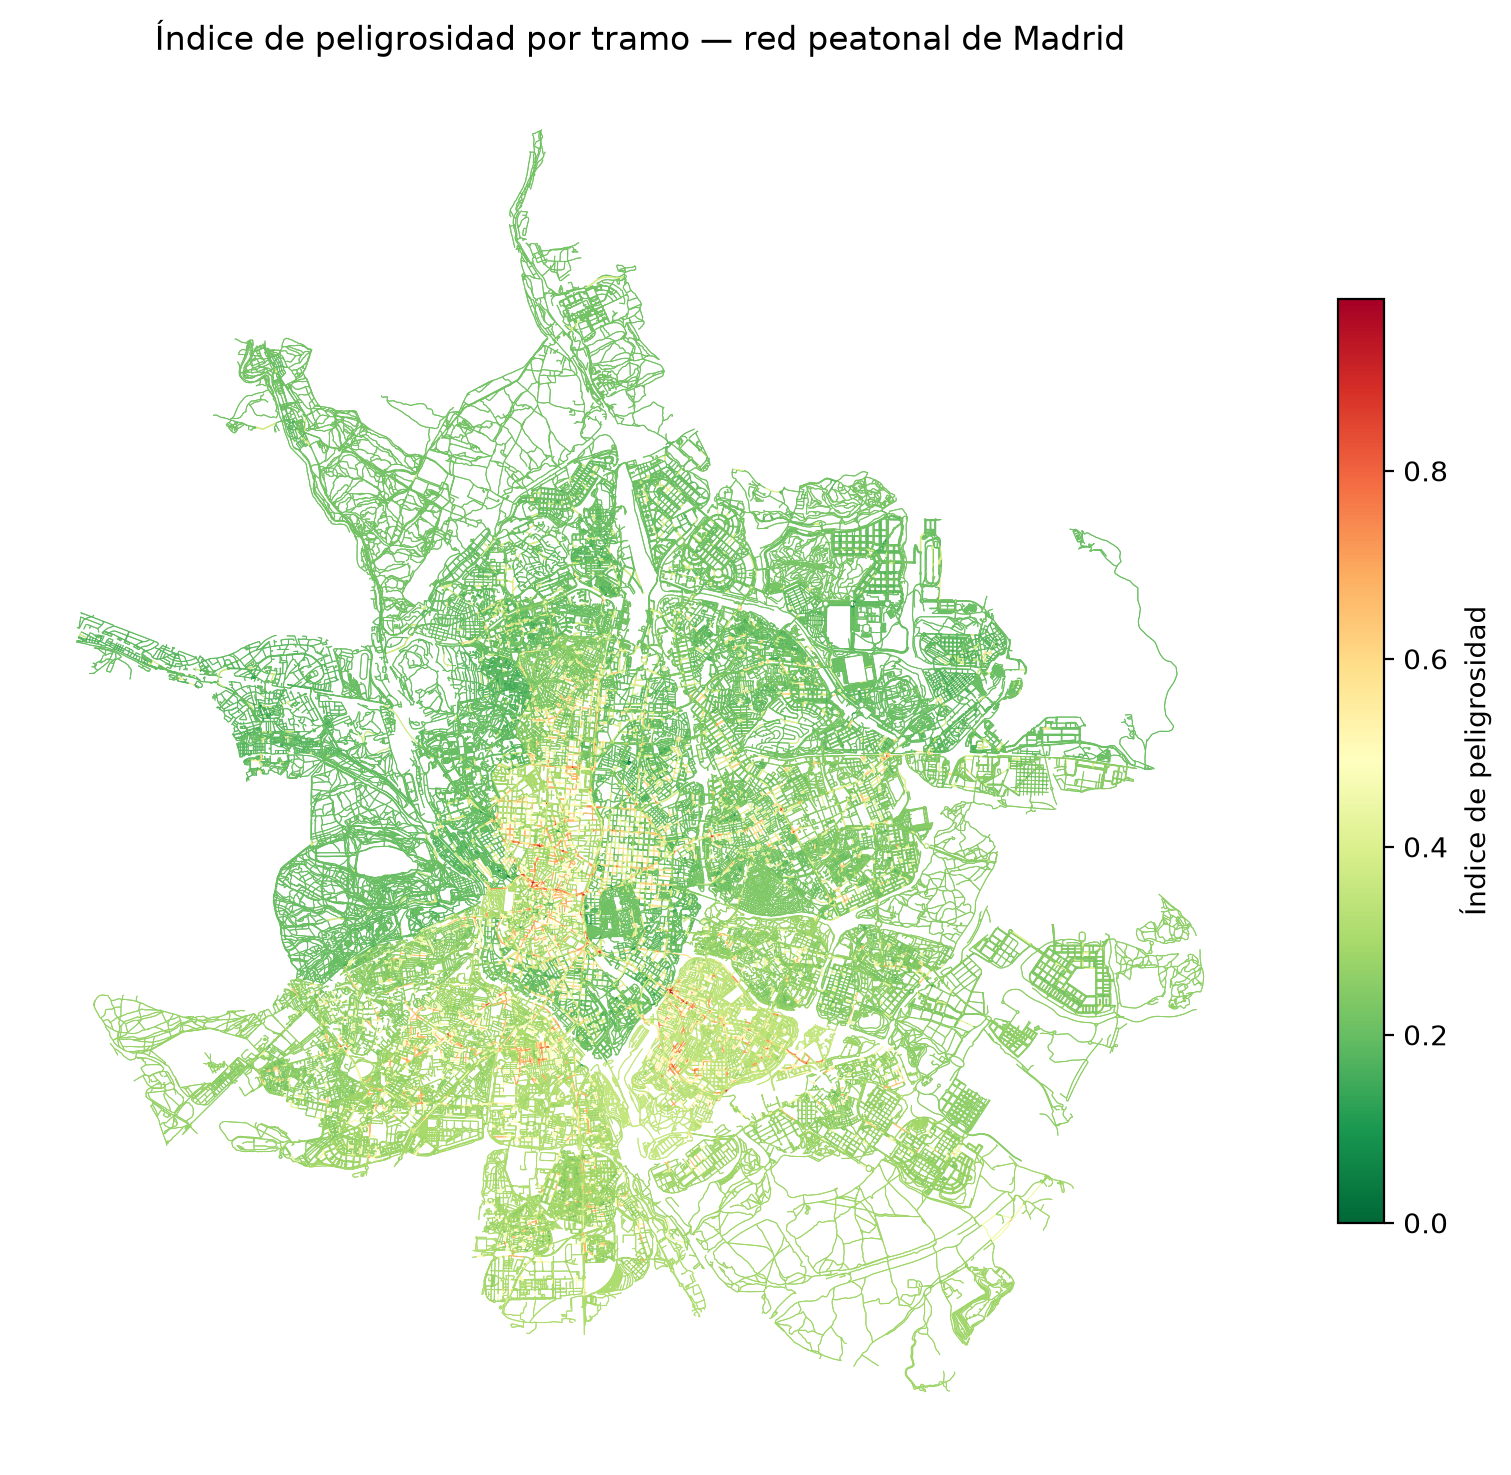
\includegraphics[width=0.8\textwidth]{imagenes/mapa_peligrosidad.png}
\caption{Índice de peligrosidad $p(e)$ por tramo en la red peatonal de Madrid (amarillo pálido: bajo, rojo oscuro: alto). Generado por \texttt{scripts/10\_mapa\_peligrosidad.py}.}
\label{fig:mapa_peligrosidad}
\end{figure}

% -----------------------------------------------------------------------
% 3.6 IMPLEMENTACIÓN DEL ENRUTAMIENTO
% -----------------------------------------------------------------------
\section{Implementación del enrutamiento seguro}
\label{sec:enrutamiento}

Una vez calculado el coste seguro para todas las aristas del grafo (Sección~\ref{subsec:coste_enrutamiento}), el enrutamiento se implementa mediante la función \texttt{pgr\_dijkstra} de pgRouting. Esta función recibe como entrada el grafo ponderado (en forma de consulta SQL sobre la tabla de aristas con sus columnas de coste), el identificador del nodo origen y el del nodo destino, y devuelve la secuencia de aristas que forman el camino de coste mínimo.

Antes de invocar \texttt{pgr\_dijkstra} es necesario resolver los dos puntos que introduce el usuario (un par de coordenadas de longitud y latitud) al nodo de la red más cercano. Esta operación se resuelve con el operador de vecino más cercano de PostGIS sobre la tabla \texttt{nodes}:

\begin{lstlisting}[style=SQL, caption={Nodo de la red más cercano a un punto dado.}, label={lst:nodo-cercano}]
SELECT osmid FROM nodes
ORDER BY geom <-> ST_SetSRID(ST_MakePoint(:lon, :lat), 4326)
LIMIT 1;
\end{lstlisting}

La consulta de enrutamiento propiamente dicha tiene la siguiente estructura:

\begin{lstlisting}[style=SQL, caption={Consulta pgRouting para el cálculo de la ruta segura, acotada a la ventana geográfica de origen y destino.}, label={lst:pgrouting}]
SELECT r.edge, e.geom, e.length, e.indice_peligrosidad
FROM pgr_dijkstra(
    -- :query construye en Python la consulta de aristas ya con
    -- la ventana geográfica (lon_min, lat_min, lon_max, lat_max
    -- y margen) resuelta a valores concretos, p. ej.:
    -- 'SELECT id, source, target, cost_seguro AS cost,
    --         reverse_cost_seguro AS reverse_cost
    --  FROM edges
    --  WHERE geom && ST_Expand(ST_MakeEnvelope(
    --      lon_min, lat_min, lon_max, lat_max, 4326), margen)'
    :query,
    :origen_id, :destino_id,
    directed => false
) r
JOIN edges e ON e.id = r.edge
ORDER BY r.seq;
\end{lstlisting}

El parámetro \texttt{directed => false} indica que el grafo se trata como no dirigido (Sección~\ref{sec:modelado_red}), por lo que \texttt{pgr\_dijkstra} puede recorrer cada arista en cualquier sentido usando indistintamente \texttt{cost} o \texttt{reverse\_cost} —en este sistema, siempre iguales—. Las filas resultantes se agregan en Python para reconstruir la geometría completa de la ruta y calcular sus estadísticas agregadas: distancia total, duración estimada (a una velocidad peatonal de referencia de 5\,km/h) y una media ponderada por longitud del índice de peligrosidad y del resto de indicadores de cada tramo recorrido.

Para el cálculo de la ruta más corta convencional (usada como referencia comparativa en el visor y en la validación), se utiliza la misma función pero sustituyendo las columnas de coste seguro por \texttt{cost} y \texttt{reverse\_cost}, que contienen directamente la longitud del tramo sin penalización alguna.

\subsection{Acotación geográfica de la consulta y elección del algoritmo}
\label{subsec:optimizacion_enrutamiento}

La primera versión de la consulta anterior no incluía la cláusula \texttt{WHERE}: se le pasaba a \texttt{pgr\_dijkstra} la red completa (\texttt{SELECT id, source, target, cost, reverse\_cost FROM edges}, sin condición alguna), delegando en el propio algoritmo la tarea de ignorar las zonas irrelevantes del grafo. Medido con \texttt{EXPLAIN ANALYZE} sobre la base de datos del proyecto (174\,394 nodos, 524\,292 aristas), esa consulta sin acotar tarda entre 1,5 y 1,9\,s por criterio, independientemente de lo corta que sea la ruta resultante, porque \texttt{pgr\_dijkstra} debe leer y materializar las 524\,292 filas de \texttt{edges} en cada invocación antes de empezar siquiera a buscar el camino.

La solución adoptada acota esa consulta a una ventana geográfica alrededor de origen y destino, apoyándose en el índice espacial \texttt{idx\_edges\_geom} (Sección~\ref{sec:modelado_red}) mediante el operador de solapamiento \texttt{\&\&}: el margen de la ventana es como mínimo de $0{,}01^\circ$ (aproximadamente 1\,km) y crece proporcionalmente a la distancia entre los dos puntos, para dar margen suficiente a los desvíos que introduce el criterio de ruta segura. Si la ventana excluyera por error el único camino posible entre dos puntos —por ejemplo, un cruce obligatorio muy alejado de la línea recta entre origen y destino—, \texttt{calcular\_ruta()} repite la consulta sin acotar antes de concluir que no existe ruta, de modo que la optimización nunca puede producir un resultado peor que antes, como mucho más lento en ese caso límite. Se comprobó, comparando la secuencia exacta de tramos devuelta con y sin acotar sobre varios pares origen-destino de distinta longitud, que ambas versiones producen la misma ruta; la acotación solo reduce el volumen de datos que \texttt{pgr\_dijkstra} tiene que leer, sin alterar el resultado. El efecto en los tiempos medidos es sustancial:

\begin{table}[h]
\centering
\begin{tabular}{lrr}
\hline
\textbf{Trayecto} & \textbf{Sin acotar} & \textbf{Acotado} \\
\hline
Corto (Puerta del Sol -- Atocha, 1,9\,km) & 1,5\,s & 0,1--0,3\,s \\
Largo (10,8\,km) & 1,9\,s & 0,7\,s \\
\hline
\end{tabular}
\caption{Tiempo de ejecución de \texttt{pgr\_dijkstra} con y sin acotar la consulta de aristas, por criterio de coste.}
\label{tab:optimizacion_dijkstra}
\end{table}

Antes de adoptar esta solución se evaluó también sustituir \texttt{pgr\_dijkstra} por \texttt{pgr\_aStar}, la variante de pgRouting que incorpora la heurística de distancia en línea recta descrita en la Sección~\ref{subsec:grafos} (dado que el coste seguro nunca es inferior a la longitud real del tramo —Sección~\ref{subsec:coste_enrutamiento}—, esa heurística es admisible también para el criterio de ruta segura, y \texttt{pgr\_aStar} garantiza por tanto encontrar la misma ruta óptima). Sin embargo, medido sobre los mismos trayectos, \texttt{pgr\_aStar} resultó sistemáticamente más lento que \texttt{pgr\_dijkstra}, tanto acotado (0,2\,s frente a 0,1\,s) como sin acotar (2,3\,s frente a 1,5\,s): \texttt{pgr\_aStar} necesita además las coordenadas de los nodos de cada arista para evaluar la heurística, lo que obliga a añadir dos \texttt{JOIN} contra la tabla \texttt{nodes} en la consulta de entrada, y ese coste adicional supera con creces el ahorro de explorar menos nodos durante la búsqueda. En otras palabras: el cuello de botella de este sistema nunca fue el algoritmo de búsqueda en sí, sino el volumen de datos que hay que leer antes de poder empezar a buscar, por lo que se mantiene \texttt{pgr\_dijkstra} y se opta por acotar la consulta de entrada en lugar de cambiar de algoritmo.

% -----------------------------------------------------------------------
% 3.7 PROTOTIPO DEL VISOR CARTOGRÁFICO
% -----------------------------------------------------------------------
\section{Prototipo del visor cartográfico}
\label{sec:visor}

El prototipo de visor cartográfico se desarrolla como una aplicación web de una sola página (\textit{Single Page Application}) utilizando \textbf{Leaflet} como biblioteca de mapas. La arquitectura del prototipo es la siguiente:

\begin{itemize}
    \item \textbf{Frontend}: página HTML con JavaScript que carga el mapa base de OpenStreetMap mediante Leaflet y ofrece tres formas de indicar el origen y el destino: un buscador de direcciones con autocompletado, un botón de geolocalización del navegador, y clic directo sobre el mapa (con geocodificación inversa para mostrar la dirección resultante). Las peticiones al backend se realizan mediante llamadas \texttt{fetch} asíncronas.
    \item \textbf{Backend}: servidor ligero en Python (Flask) con tres rutas: \texttt{GET /api/ruta}, que recibe las coordenadas de origen y destino, resuelve los nodos más cercanos, lanza las dos consultas de enrutamiento (segura y rápida) contra la base de datos y devuelve las geometrías resultantes en GeoJSON junto con sus estadísticas; y \texttt{GET /api/geocode} y \texttt{GET /api/geocode/inverso}, que actúan como \textit{proxy} de los servicios de geocodificación CartoCiudad (IGN) y Nominatim (OpenStreetMap), evitando exponer directamente esos servicios externos al cliente.
    \item \textbf{Visualización}: el visor ofrece dos modos de uso, seleccionables por el usuario. En el modo \textbf{simple} se dibuja únicamente la ruta segura, con su distancia, duración estimada y una insignia cualitativa del nivel de seguridad (obtenida discretizando el índice de peligrosidad medio de la ruta). En el modo \textbf{detallado} se dibujan ambas rutas sobre el mapa —en verde la segura, en azul discontinuo la rápida— junto con una tabla comparativa tramo a tramo de todos los indicadores descritos en la Sección~\ref{sec:funcion_coste} (siniestralidad, atropellos, iluminación y vulnerabilidad), señalando en qué medida la ruta segura mejora o empeora cada uno respecto a la ruta rápida.
\end{itemize}

A diferencia del planteamiento inicial, el prototipo implementado \textbf{no incluye un selector de franja horaria}, de forma coherente con la ausencia de esa dimensión en la función de coste (Sección~\ref{sec:vision_general}).